\section{Cross Validation}
With CV we want to solve a problem we introduce with the split in training and test data.  One problem with this approach is the following: If we select 20\% (or some other fraction) for testing, then the test-error depends on a (potentially small) random set. For a different set, we could get a different test-error. $\rightarrow$ CV is a technique to compare (and select from) different models (=different parameter values) \textbf{Use Cases:} estimation of generalization error, selection of hyper parameters.

\subsection{k-Cross Validation}
\begin{minipage}{0,5\linewidth}
	We can apply cv to obtain a better estimate of the generalization error.\\
	In k-fold cross-validation, we repeat the split-train-test procedure k times, using a systematic resampling procedure.\\
	The data is split once into k folds. Then train/test is repeated k-times. Each fold participates in k-1 training phases and is used once for testing:
 
\end{minipage}
\begin{minipage}{0,5\linewidth}
	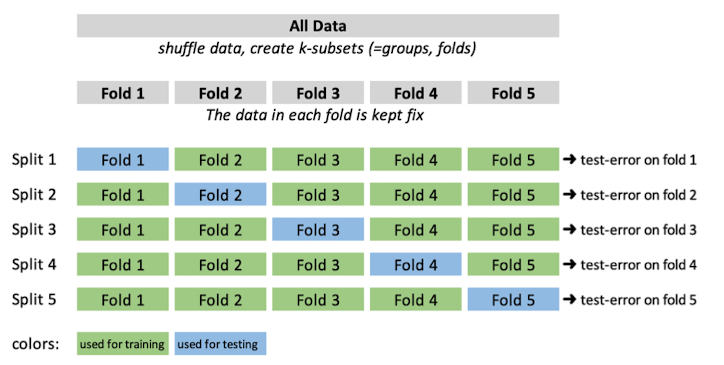
\includegraphics[width=\linewidth]{k-fold}
\end{minipage}

\subsection{Selection of Hyper Parameters}
The split/train pattern of cross validation can be used to find optimal hyper parameters.

\section{Artificial Neural Networks}
\subsection{Neuron}
\begin{minipage}{0,5\linewidth}
	The artificial neuron receives an input vector $[x_{1},x_{2},x_{3},...]$. Each neuron has its own input weights $[w_{1},w_{2},w_{3},...]$ and bias $b (=intercept)$.
	
	The neuron calculates the sum of the weighted input (dot product $\vec{x} * \vec{w}$), adds a bias b, and passes it through a nonlinear activation function (=only positive values pass).
\end{minipage}
\begin{minipage}{0,5\linewidth}
	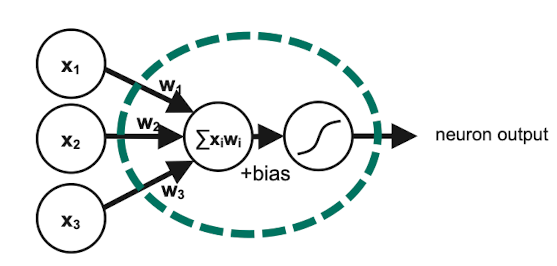
\includegraphics[width=\linewidth]{neuron}
\end{minipage}

\subsection{Artificial Neuron Network (ANN)}
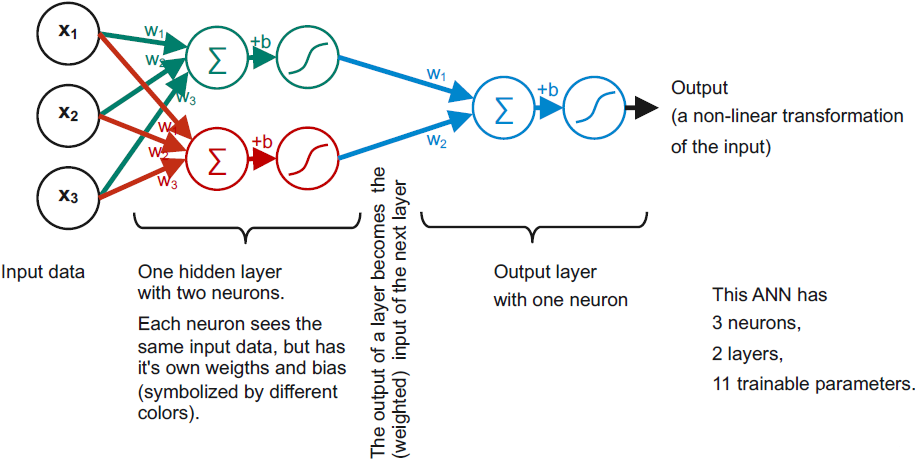
\includegraphics[width=\linewidth]{ANN_2}

\subsection{How to train a ANN}
 We consider a simple case of supervised learning: for each input we are given the output (target values/labels). The ANN is initialized with random weights and produces some output  $\hat{y}$. Then, an optimizer (e.g. SGD) reduces a cost-function (e.g. MSE).
 
  That is, at every iteration, and for every single weight w (\& and every bias b), the partial derivative $\frac{\partial }{\partial w} (y-\hat{y})^2$ needs to be calculated. Luckily there's an algorithm which is doing this very efficiently: \textbf{Backpropagation}.



